    % CVPR 2022 Paper Template
% based on the CVPR template provided by Ming-Ming Cheng (https://github.com/MCG-NKU/CVPR_Template)
% modified and extended by Stefan Roth (stefan.roth@NOSPAMtu-darmstadt.de)

\documentclass[10pt,twocolumn,letterpaper]{article}

%%%%%%%%% PAPER TYPE  - PLEASE UPDATE FOR FINAL VERSION
% \usepackage[review]{cvpr}      % To produce the REVIEW version
% \usepackage{cvpr}              % To produce the CAMERA-READY version
\usepackage[pagenumbers]{cvpr} % To force page numbers, e.g. for an arXiv version

% Include other packages here, before hyperref.
\usepackage{graphicx}
\usepackage{amsmath}
\usepackage{amssymb}
\usepackage{bm}
\usepackage{booktabs}

% Figures live in report/figures/, one level up from report/latex/.
\graphicspath{{../figures/}}


% It is strongly recommended to use hyperref, especially for the review version.
% hyperref with option pagebackref eases the reviewers' job.
% Please disable hyperref *only* if you encounter grave issues, e.g. with the
% file validation for the camera-ready version.
%
% If you comment hyperref and then uncomment it, you should delete
% ReviewTempalte.aux before re-running LaTeX.
% (Or just hit 'q' on the first LaTeX run, let it finish, and you
%  should be clear).
\usepackage[pagebackref,breaklinks,colorlinks]{hyperref}


% Support for easy cross-referencing
\usepackage[capitalize]{cleveref}
\crefname{section}{Sec.}{Secs.}
\Crefname{section}{Section}{Sections}
\Crefname{table}{Table}{Tables}
\crefname{table}{Tab.}{Tabs.}


%%%%%%%%% PAPER ID  - PLEASE UPDATE
\def\cvprPaperID{*****} % *** Enter the your report id
\def\confName{CVPR}
\def\confYear{2022}


\begin{document}

%%%%%%%%% TITLE - PLEASE UPDATE
\title{DribbleAMP: Adversarial Motion Priors for Football Dribbling}

\author{Eryk Halicki\\
ETH Z\"urich\\
{\tt\small ehalicki@ethz.ch}
\and
Jay Janaskar\\
ETH Z\"urich\\
{\tt\small jjanaskar@ethz.ch}
}
\maketitle

%%%%%%%%% ABSTRACT
\begin{abstract}
   We present \textbf{DribbleAMP}, a physics-based controller that learns to
   dribble a football while preserving natural, human-like locomotion. Building
   on Adversarial Motion Priors (AMP), we replace hand-crafted style penalties
   with a learned style reward from unlabeled locomotion clips and add a
   velocity-conditioned task reward: the agent must drive the ball so its ground
   velocity matches a continuously re-sampled target direction and speed while
   staying near the ball. A two-phase curriculum first teaches the agent to
   approach and kick the ball, then to steer it. We train in the Newton GPU
   simulator with $1024$ parallel environments on both a generic humanoid and a
   simulated Unitree G1, obtaining policies that track commanded ball velocities
   while remaining visually natural. Code:
   \url{https://github.com/ErykHalicki/DribbleAMP}.
\end{abstract}

%%%%%%%%% BODY TEXT
\section{Introduction}
\label{sec:intro}

\paragraph{Goal and motivation.}
We train a human-like, continuous football-dribbling policy for a simulated
humanoid, including the Unitree G1, by combining Adversarial Motion
Priors~\cite{peng2021amp} with a ball-velocity command. Dribbling is a demanding
benchmark for whole-body humanoid control: it couples locomotion, balance, and
contact-rich interaction with an external, under-actuated object. Robust and
\emph{natural} locomotion is a prerequisite for deploying humanoids in the real
world, and dribbling has a direct application in RoboCup-style humanoid soccer.

\paragraph{Why existing methods fall short.}
Pure task-reward RL can move the ball but tends to produce unnatural,
energy-inefficient gaits. Motion-tracking methods such as
DeepMimic~\cite{peng2018deepmimic} reproduce reference clips faithfully but
require a motion that already \emph{contains} the dribble, which is hard to
capture and does not generalize to arbitrary commanded directions. The closest
prior work, DribbleMaster~\cite{dribblemaster}, achieves strong sim-to-real
dribbling but relies on hand-crafted style penalties (torso tilt, a gait clock,
reference tracking) and is not open-sourced.

\paragraph{Our solution.}
We pose dribbling as \emph{velocity-conditioned} control and build an
AMP\,$\times$\,DribbleMaster hybrid: AMP's learned discriminator replaces
DribbleMaster's hand-crafted style penalties, supplying a style prior from
generic walking/running clips, while we adapt DribbleMaster's task-reward design
into a three-term ball reward. A two-phase curriculum decouples ``learn to
approach and kick the ball'' from ``learn to steer it,'' yielding natural gaits
\emph{and} directional ball control without any dribbling reference motion.

\paragraph{Contributions.}
\begin{enumerate}
    \item A velocity-conditioned dribbling task and a three-term ball reward
    (\cref{sec:reward}) integrated into the AMP framework, on both a generic
    humanoid and the Unitree G1.
    \item A two-phase chase-then-dribble curriculum (\cref{sec:curriculum}) and
    an ablation measuring how much it actually helps.
    \item An open-source implementation on top of MimicKit~\cite{mimickit2025}
    with the Newton GPU backend, with reward-design and training-budget lessons.
\end{enumerate}

%-
%------------------------------------------------------------------------
\section{Related Work}
\label{sec:relatedwork}

% --- OUTLINE: group by topic, end each group with how we differ. ---
\paragraph{Motion imitation for physics-based control.}
DeepMimic~\cite{peng2018deepmimic} and follow-ups track reference clips with a
phase-indexed tracking reward. They produce high-quality motion but require a
reference that already demonstrates the target skill. We instead need a
\emph{skill not present} in any clip (ball dribbling), so direct imitation does
not apply.

\paragraph{Adversarial motion priors.}
AMP~\cite{peng2021amp} replaces the tracking reward with a discriminator-based
\emph{style} reward learned from an unstructured motion dataset, producing
natural motion with no motion planner and freeing the task reward to specify
only the goal. We use AMP as our backbone and contribute the task definition,
reward, and curriculum on top of it.

\paragraph{Learning to dribble.}
DribbleMaster~\cite{dribblemaster} learns RL humanoid dribbling with sim-to-real
transfer using hand-crafted style penalties and a two-stage curriculum, with
strong results, but its code is not open-sourced, which limits direct
comparison. We reuse its task-reward blueprint but obtain style from an AMP
discriminator instead of hand-designed penalties, and target a
\emph{velocity-conditioned} command (direction + speed) rather than a positional
goal.

\paragraph{Simulation \& frameworks.}
We build on MimicKit~\cite{mimickit2025}, an open-source imitation-plus-RL
framework that supports AMP and the Unitree G1 on Isaac Gym and Isaac Lab; we
add our task on top of it. We train with massively parallel GPU simulation
(Newton, and Isaac Gym~\cite{makoviychuk2021isaacgym}-style throughput) using
PPO~\cite{schulman2017ppo} as the RL optimizer.


\section{Method}
\label{sec:method}

\subsection{Preliminaries: AMP}
We adopt the AMP formulation~\cite{peng2021amp}: the agent maximizes a convex
combination of a task (goal) reward $r_\text{task}$ and a learned style reward
$r_\text{style}$,
\begin{equation}
    r_\text{total} = w_\text{task}\, r_\text{task} + w_\text{style}\, r_\text{style},
\end{equation}
where $r_\text{style}$ is produced by a discriminator trained to separate policy
motion from an unlabeled motion dataset. This discriminator replaces
DribbleMaster's hand-crafted style penalties (torso tilt, gait clock, reference
tracking). As the motion dataset we use the existing G1 and humanoid retargeted
locomotion clips (walk, run) shipped with MimicKit; no dribbling reference
motion is needed. We set $(w_\text{task},w_\text{style})=(0.8,0.2)$ in the
dribble phase. The remainder of this section specifies $r_\text{task}$.

\subsection{Task setup and observations}
The character (a generic humanoid, or the Unitree G1) is initialized next to a
free-rolling ball. The task is defined by a \emph{target ball velocity}: a unit
direction $\hat{\mathbf{d}}^*$ and a target speed $s^*$, both re-sampled at
random intervals (every $4$--$7$\,s) during an episode. The policy observes, in
the character's heading frame, proprioception plus the local ball position and
velocity and the target direction and speed, appended to the standard AMP
observation.

\subsection{Reward formalization}
\label{sec:reward}

% ====================================================================
% Reward formalization (ported from report/soccer_reward.tex).
% Matches compute_soccer_reward() in
% MimicKit/mimickit/envs/task_soccer_env.py.
% ====================================================================

\paragraph{Notation.}
\begin{itemize}
    \item $\mathbf{p}_b \in \mathbb{R}^2$: ball position (xy-plane)
    \item $\mathbf{v}_b \in \mathbb{R}^2$: ball velocity (xy-plane)
    \item $\mathbf{p}_c \in \mathbb{R}^2$: character root position (xy-plane)
    \item $\hat{\mathbf{d}}^* \in \mathbb{R}^2$: target ball direction (unit vector)
    \item $s^* \in \mathbb{R}_{\geq 0}$: target ball speed
    \item $w_s, w_d, w_r$: weights for the speed, direction, and distance terms
    \item $\sigma_s, \sigma_r$: scale factors for the speed and distance terms
    \item $\varepsilon = 10^{-6}$: numerical stabiliser
\end{itemize}

\paragraph{Speed reward.} Penalises deviation of the ball speed from the target:
\begin{equation}
    r_s = \exp\!\left(-\sigma_s \, \bigl(s^* - \|\mathbf{v}_b\|\bigr)^2\right).
\end{equation}

\paragraph{Direction reward.} Rewards alignment of the ball velocity with the
target direction:
\begin{equation}
    r_d = \max\!\left(0,\; \frac{\mathbf{v}_b}{\|\mathbf{v}_b\| + \varepsilon} \cdot \hat{\mathbf{d}}^*\right).
\end{equation}

\paragraph{Distance reward.} Encourages the character to stay close to the ball:
\begin{equation}
    r_r = \exp\!\left(-\sigma_r \, \|\mathbf{p}_b - \mathbf{p}_c\|^2\right).
\end{equation}

\paragraph{Total task reward.}
\begin{equation}
\label{eq:total-reward}
    r_\text{task} = w_s \, r_s + w_d \, r_d + w_r \, r_r,
\end{equation}
or equivalently,
\begin{equation}
\begin{aligned}
    r_\text{task} =\;
      &\underbrace{w_s \exp\!\bigl(-\sigma_s (s^* - \|\mathbf{v}_b\|)^2\bigr)}_{\text{speed}}
      + \underbrace{w_d \max\!\left(0,\; \tfrac{\mathbf{v}_b \cdot \hat{\mathbf{d}}^*}{\|\mathbf{v}_b\| + \varepsilon}\right)}_{\text{direction}}\\[-0.3em]
      &+ \underbrace{w_r \exp\!\bigl(-\sigma_r \|\mathbf{p}_b - \mathbf{p}_c\|^2\bigr)}_{\text{distance}}.
\end{aligned}
\end{equation}

\subsection{Two-phase curriculum}
\label{sec:curriculum}
\Cref{eq:total-reward} is intuitively hard to optimize from scratch: the
direction term $r_d$ is uninformative until the agent already moves the ball. We
therefore split training into two stages that share the reward
\eqref{eq:total-reward} but use different weights and spawn settings:
\begin{itemize}
    \item \textbf{Stage 1 (chase).} The ball spawns far from the agent
    ($5$--$10$\,m). Only the distance and ball-speed terms are active
    ($w_d = 0$); the goal is to learn to balance, approach, and kick the ball.
    Weights $(w_s, w_d, w_r) = (0.6,\,0.0,\,0.4)$.
    \item \textbf{Stage 2 (dribble).} The ball spawns close to the agent and all
    three terms are active. This stage warm-starts from the Stage-1 checkpoint.
    Weights $(w_s, w_d, w_r) = (0.3,\,0.5,\,0.2)$.
\end{itemize}
This mirrors DribbleMaster's two-stage curriculum, which they report improves
success from $33\%$ (single-stage) to $87\%$ (two-stage). We test whether this
benefit holds in our AMP-based setup in \cref{sec:experiments}. A summary of
all reward hyper-parameters is given in \cref{tab:hparams}.

\begin{table}[t]
\centering
\caption{Reward weights and scales per phase (see \cref{sec:reward}).}
\label{tab:hparams}
\begin{tabular}{lccccc}
\toprule
Phase & $w_s$ & $w_d$ & $w_r$ & $\sigma_s$ & $\sigma_r$ \\
\midrule
1 (contact/push) & 0.6 & 0.0 & 0.4 & 0.2 & 0.1 \\
2 (steer)        & 0.3 & 0.5 & 0.2 & 0.2 & 0.1 \\
\bottomrule
\end{tabular}
\end{table}


\section{Experiments}
\label{sec:experiments}

\subsection{Setup}
We train with the Newton GPU backend using $1024$ parallel environments and the
AMP/PPO agent from MimicKit. The style dataset is the retargeted locomotion
clips (no dribbling clips). Episodes last $60$\,s in Stage~1 and $20$\,s in
Stage~2. Training is expensive: a single configuration needs roughly $12$--$24$
hours to reveal whether it worked, and with a budget of about $150$ GPU-hours
per person we could not run full hyper-parameter sweeps.

\subsection{Evaluation metrics}
We measure, over evaluation episodes: (i) \emph{speed error}
$|s^* - \|\mathbf{v}_b\||$ (m/s); (ii) \emph{angle error}, the angle between the
ball velocity and the target direction (deg); (iii) \emph{character--ball
distance} (m); and (iv) mean test return during training. We also assess gait
naturalness qualitatively from rollout videos.

\subsection{Main comparison: does the curriculum help?}
We compare three training schemes evaluated on the Stage-2 dribbling task:
\emph{Stage~1 only}, \emph{Stage~2 only} (trained from scratch on the full
reward), and \emph{Stage~1\,+\,Stage~2} (our curriculum).
\Cref{tab:ablation} reports the three error metrics, visualized in
\cref{fig:comparison}.

\begin{table}[t]
\centering
\caption{Tracking errors on the dribbling task (lower is better). Stage~1 only
never learns to steer the ball; Stage~2-only and the full curriculum are nearly
indistinguishable.}
\label{tab:ablation}
\begin{tabular}{lccc}
\toprule
Scheme & Speed err.\ & Angle err.\ & Char--ball \\
       & (m/s)       & (deg)       & dist.\ (m) \\
\midrule
Stage 1 only        & 0.917 & 81.23 & 0.782 \\
Stage 2 only        & 0.735 & 19.70 & 0.607 \\
Stage 1 + Stage 2   & \textbf{0.732} & \textbf{19.52} & \textbf{0.588} \\
\bottomrule
\end{tabular}
\end{table}

\begin{figure}[t]
\centering
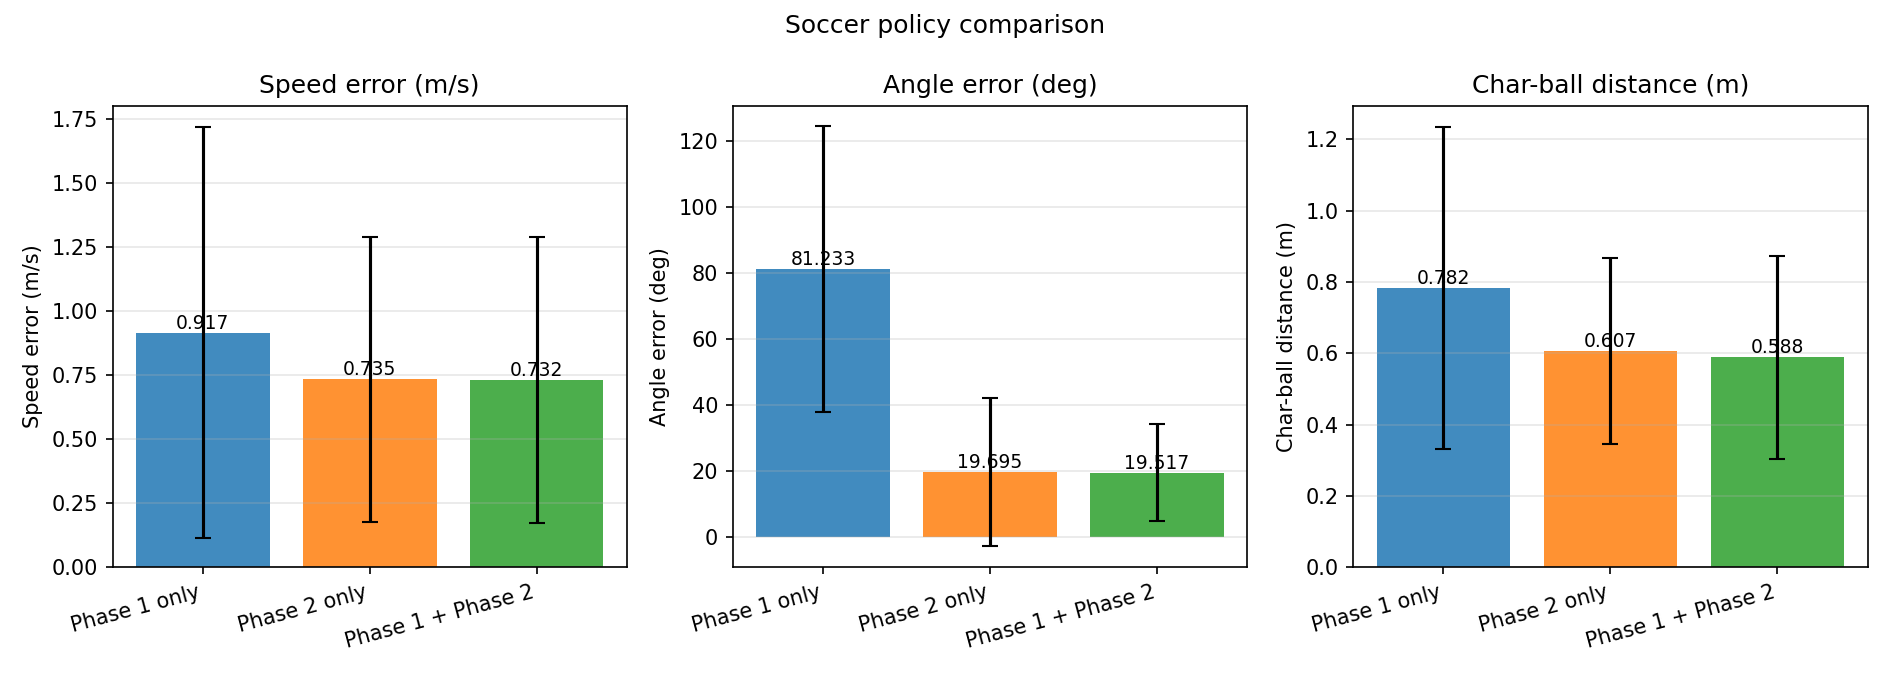
\includegraphics[width=\linewidth]{comparison.png}
\caption{Per-metric comparison of the three training schemes. Stage~1 only has a
very large angle error ($81^\circ$) since it is never rewarded for direction;
Stage~2-only and the full two-stage curriculum are essentially tied.}
\label{fig:comparison}
\end{figure}

The headline finding is that the two-stage curriculum does \emph{not}
meaningfully outperform training Stage~2 from scratch: angle error drops only
from $19.70^\circ$ to $19.52^\circ$ and speed error from $0.735$ to $0.732$\,m/s.
This contrasts with the large gap DribbleMaster reports for their curriculum,
and we attribute the difference partly to AMP's style prior already
regularizing the policy toward sensible locomotion, and partly to our inability
to tune extensively under the GPU budget. Stage~1 alone, as expected, learns to
approach and kick but not to steer ($81^\circ$ angle error).

\subsection{Ablation: AMP vs.\ no AMP}
\label{sec:ablation-amp}
To isolate the contribution of the adversarial style prior, we compare our full
model against a \emph{no-AMP} baseline that is identical in every respect ---
same environment, network, optimizer, and Stage-2 task reward --- except that
the style (discriminator) reward is removed by setting
$(w_\text{task}, w_\text{style}) = (1.0, 0.0)$. Both are trained from scratch on
the Stage-2 dribbling task. \Cref{tab:amp-ablation} reports the task-tracking
metrics together with a \emph{style score}: the average discriminator output on
each policy's motion, where higher means the locomotion looks more like the
reference clips.

\begin{table}[t]
\centering
\caption{AMP vs.\ no-AMP, both trained from scratch on the Stage-2 task. The
style score is the discriminator's mean output on the policy's motion (higher =
more natural). % TODO: fill in numbers once the no-AMP run finishes.
}
\label{tab:amp-ablation}
\begin{tabular}{lcccc}
\toprule
Model & Speed err.\ & Angle err.\ & Char--ball & Style \\
      & (m/s)       & (deg)       & dist.\ (m) & score \\
\midrule
No AMP        & TODO & TODO & TODO & TODO \\
AMP (ours)    & TODO & TODO & TODO & TODO \\
\bottomrule
\end{tabular}
\end{table}

% TODO: discuss the expected pattern once results are in: no-AMP may match or
% slightly beat AMP on raw task error while scoring far lower on style and
% producing visibly unnatural, "cheating" gaits (see Fig.~\ref{fig:no_amp_rollout}).
\Cref{fig:no_amp_rollout} shows a representative no-AMP rollout for qualitative
comparison against the AMP results in
\cref{fig:humanoid_rollout,fig:g1_rollout}.

\begin{figure}[t]
\centering
% TODO: add no_amp_rollout.png to report/figures/ once the run is trained.
% 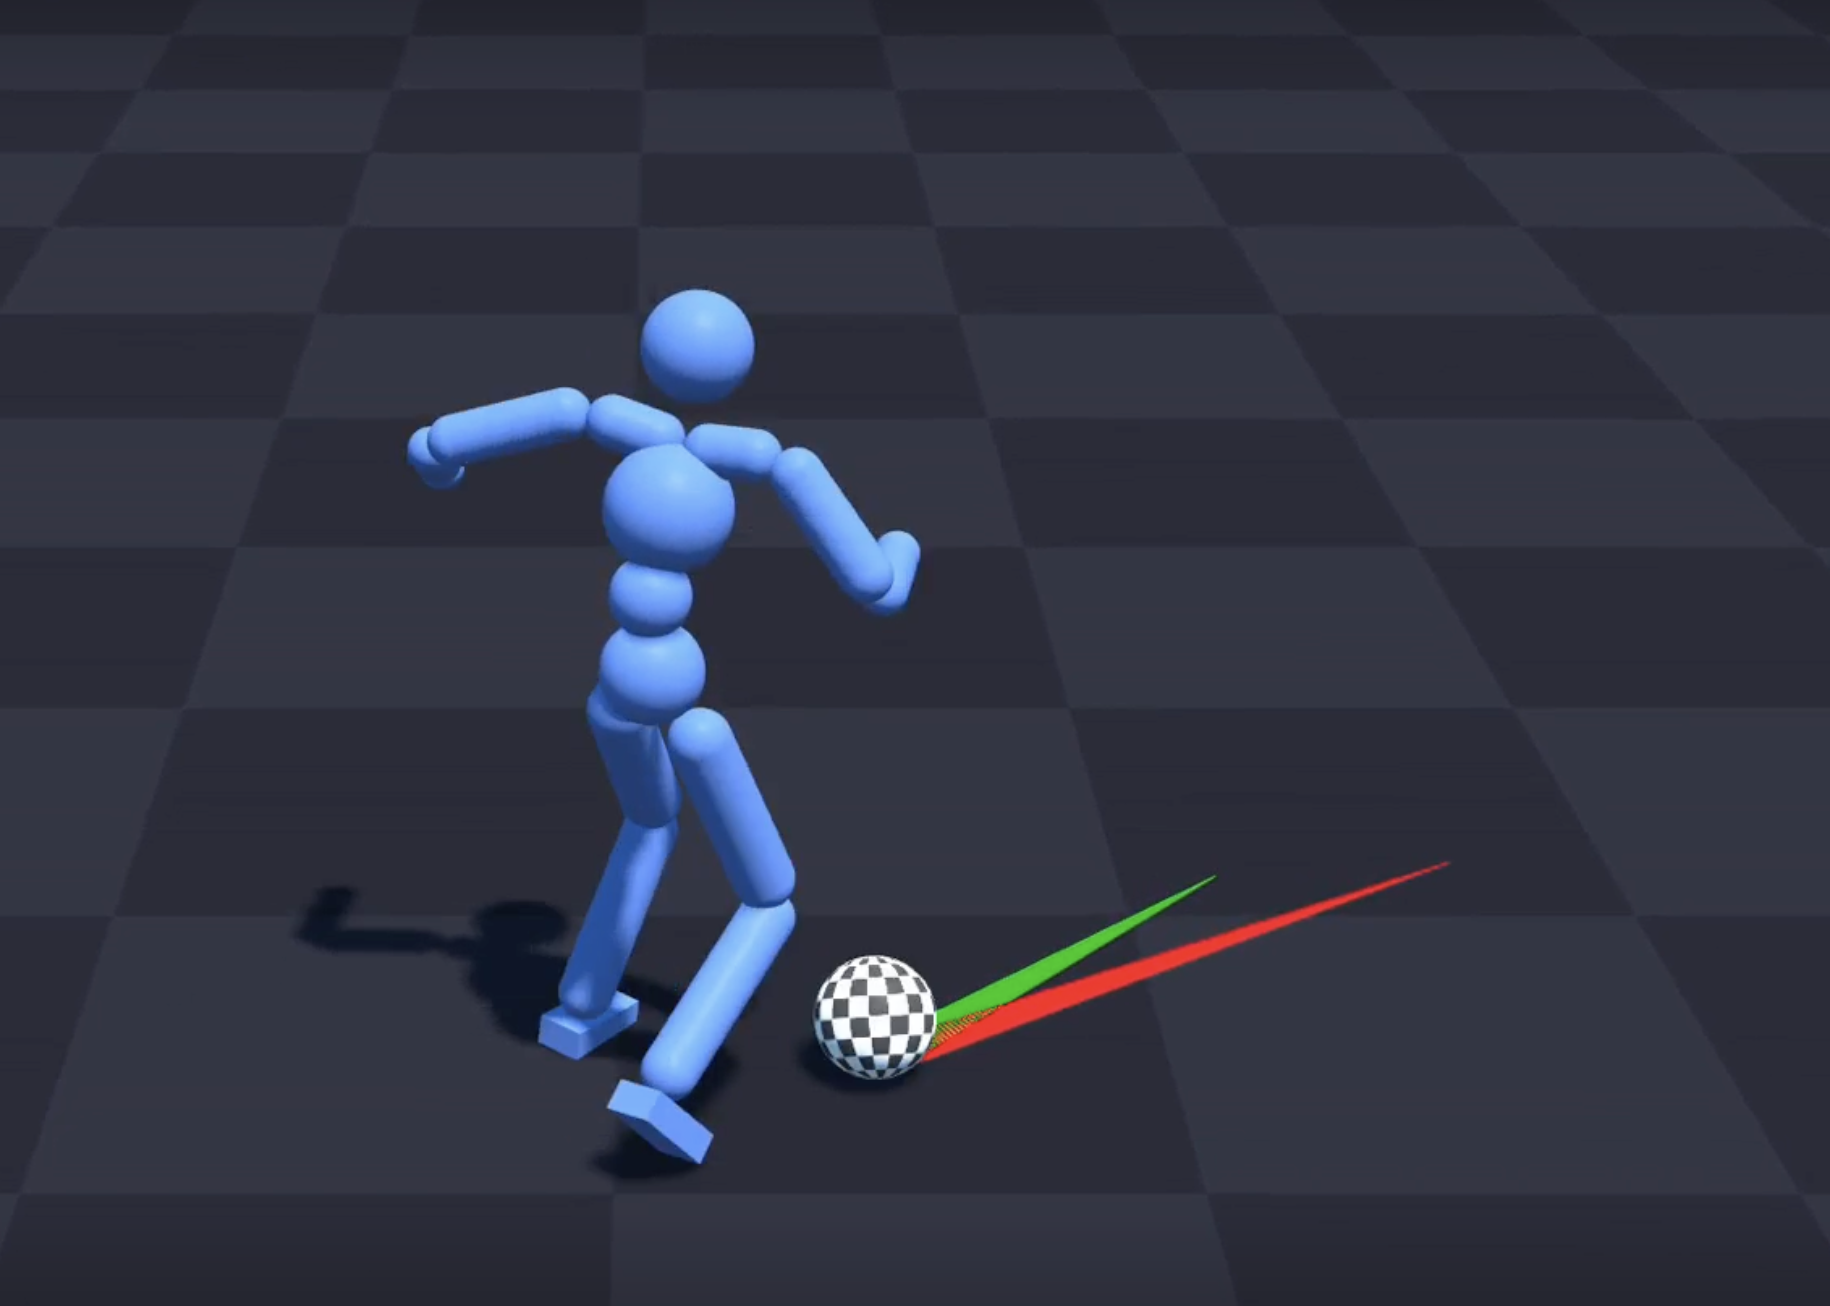
\includegraphics[width=0.85\linewidth]{no_amp_rollout.png}
\caption{No-AMP rollout (task reward only). % TODO: describe the unnatural gait
relative to the AMP policy.}
\label{fig:no_amp_rollout}
\end{figure}

\subsection{Training curves}
\Cref{fig:curves} shows test return for the two regimes. The curriculum
(Stage~1 $\approx$ 10k iters $\rightarrow$ Stage~2 $\approx$ 30k iters) peaks
around a return of $465$, while Stage~2-only ($\approx$ 25k iters) peaks around
$450$ but starts from a much lower return and climbs more steeply once it
discovers ball contact. We also trained the policy on the Unitree G1 in Newton;
training was less stable (one run dropped sharply near iteration $2200$ before
recovering) but reached a peak return of $448$ against a theoretical maximum of
$600$.

\begin{figure}[t]
\centering
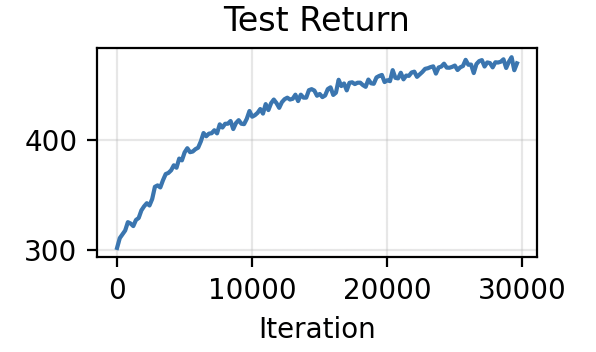
\includegraphics[width=0.49\linewidth]{phase12_humanoid_training.png}
\hfill
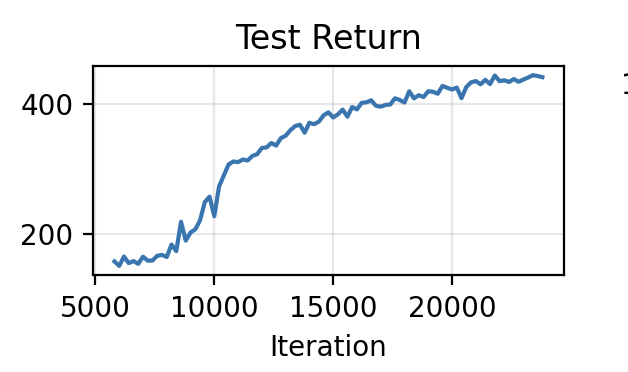
\includegraphics[width=0.49\linewidth]{phase2_only_humanoid_training.png}
\caption{Humanoid test return. Left: two-stage curriculum. Right: Stage~2 only.
Both converge to a similar final return.}
\label{fig:curves}
\end{figure}

\subsection{Qualitative results}
\Cref{fig:humanoid_rollout,fig:g1_rollout} show representative rollouts on the
generic humanoid and the Unitree G1. In both, the green arrow is the current
ball velocity and the red arrow is the commanded target velocity; their close
alignment indicates successful velocity-conditioned dribbling.

\begin{figure}[t]
\centering
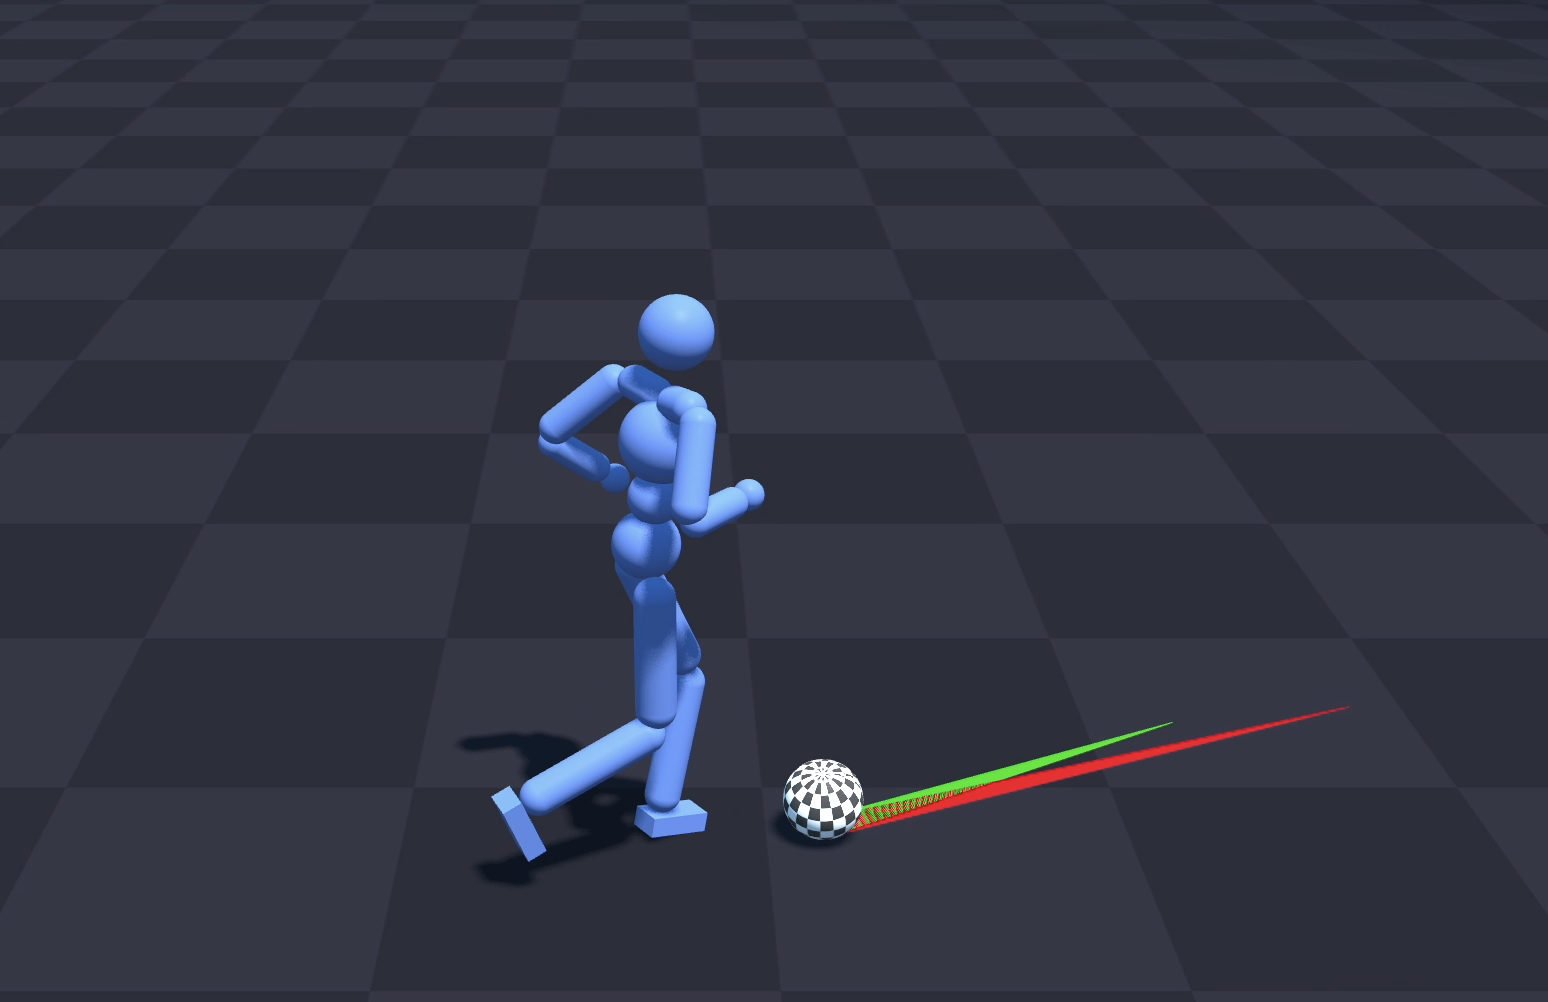
\includegraphics[width=0.85\linewidth]{humanoid_rollout.png}
\caption{Dribbling rollout on the generic humanoid. Green: current ball
velocity; red: commanded target velocity.}
\label{fig:humanoid_rollout}
\end{figure}

\begin{figure}[t]
\centering
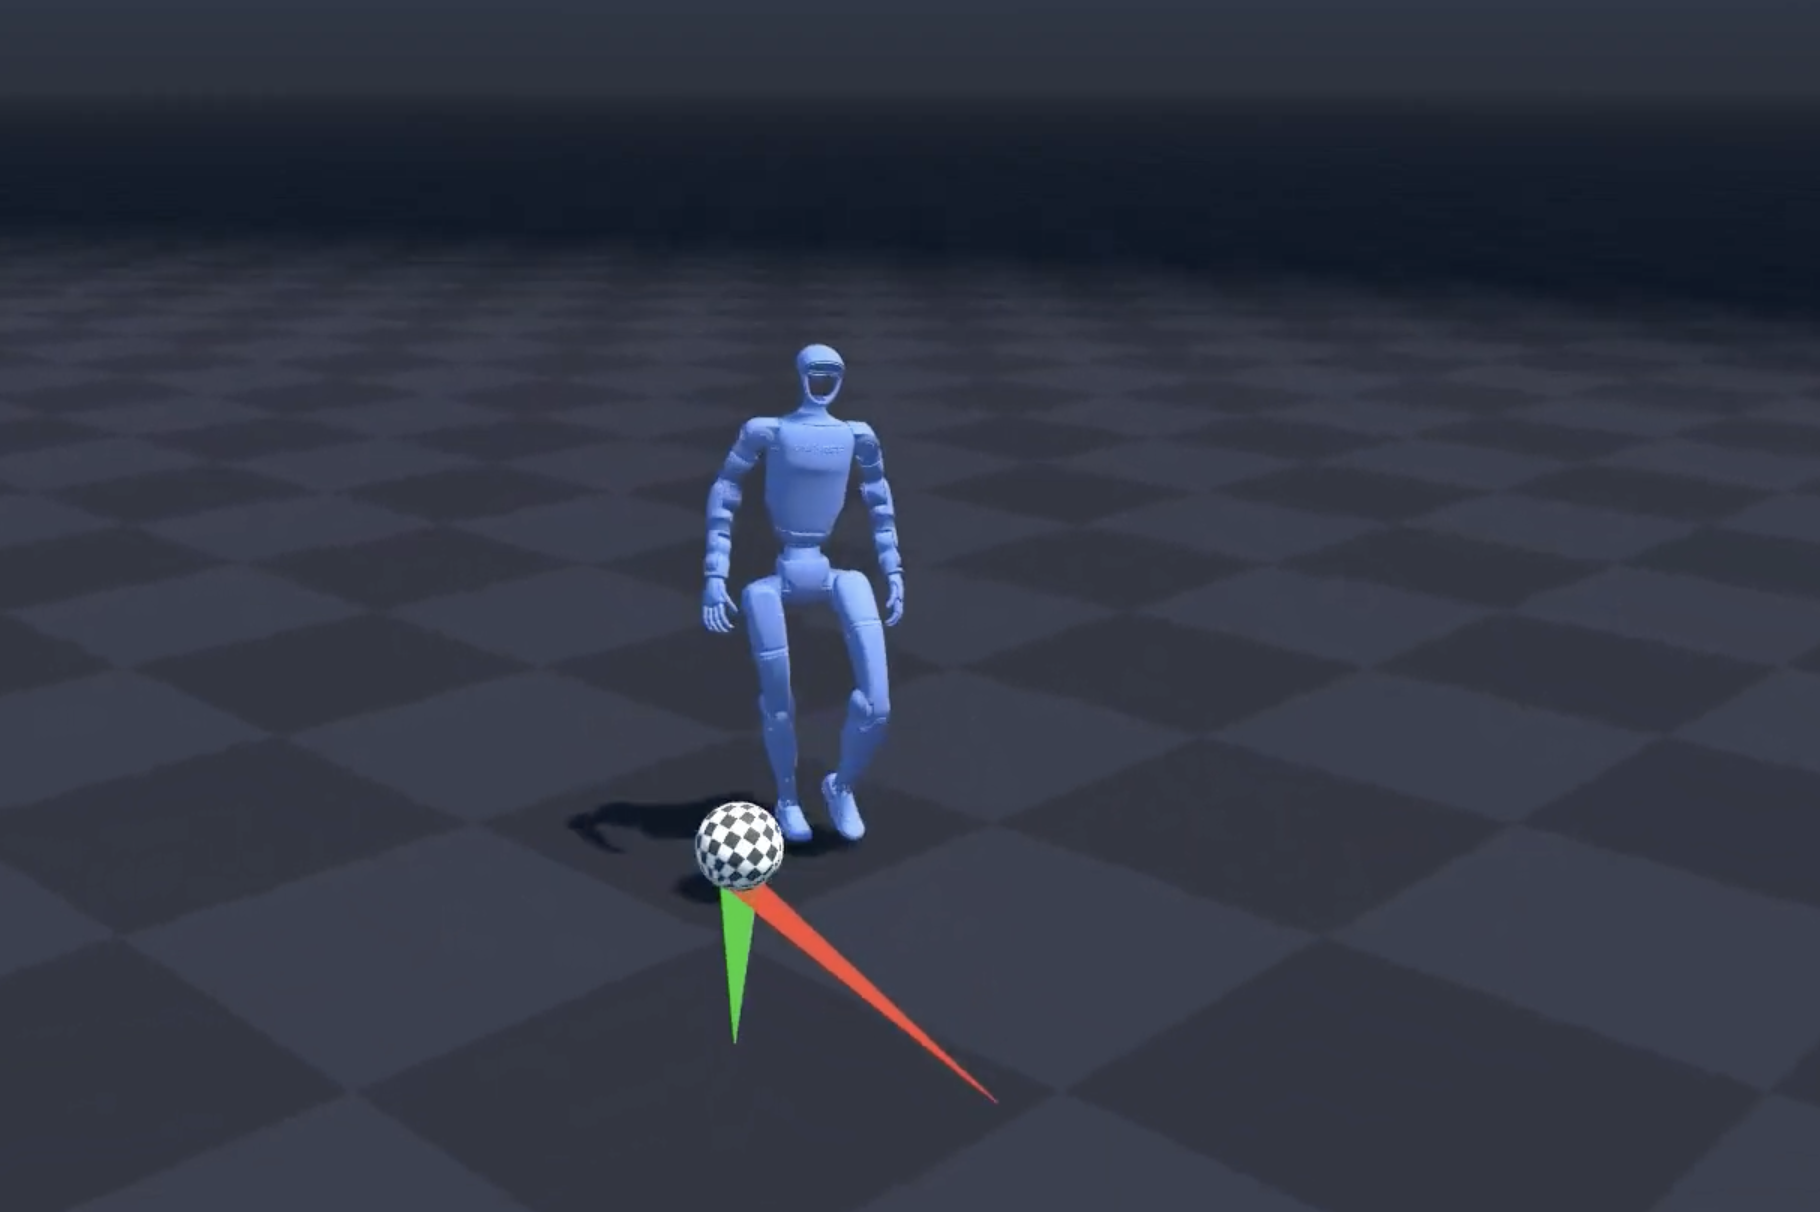
\includegraphics[width=0.85\linewidth]{g1_rollout.png}
\caption{Dribbling rollout on the Unitree G1. Green: current ball velocity;
red: commanded target velocity.}
\label{fig:g1_rollout}
\end{figure}

\subsection{Failure cases and challenges}
Reward design was the dominant difficulty. When the weights are poorly tuned,
the agent either never learns to approach the ball or learns to walk in circles
around it. If the discriminator (style) weight is too high, the policy is pulled
toward a clean walking gait, which is sub-optimal for the contact-rich motion
dribbling requires. Combined with the $12$--$24$\,h turnaround per configuration
and a limited GPU budget, this made tuning slow. Finally, because
DribbleMaster's code is not open-sourced, we cannot provide a fully controlled
head-to-head comparison.


\section{Conclusion}
\label{sec:conclusion}

\paragraph{Summary.}
We posed humanoid football dribbling as velocity-conditioned control and solved
it with an AMP\,$\times$\,DribbleMaster hybrid that obtains style from a learned
discriminator instead of hand-crafted penalties. The resulting policies track
commanded ball velocities while remaining visually natural, on both a generic
humanoid and the Unitree G1. Our ablation shows that, in this AMP-based setup,
the two-stage curriculum gives only a marginal improvement over training the
full reward directly --- a useful negative result given the cost of the extra
stage.

\paragraph{Limitations.}
We evaluate a single ball on flat ground with no opponents, and steering is
velocity-conditioned only. All results are in simulation; we did not perform
sim-to-real transfer. Limited GPU budget prevented systematic reward tuning.

\paragraph{Future work.}
Promising directions include a vision-based, end-to-end policy that replaces the
oracle ball position with visual input (currently limited by MimicKit's lack of
support for CNN/Transformer policies), sim-to-real transfer to real G1 hardware,
a controlled baseline against DribbleMaster should its code be released, and
retargeting motion clips from real soccer players to improve dribbling style.

\section{Contributions of team members}
Both authors contributed to report writing, the presentation, and model training
and evaluation. \textbf{Eryk Halicki} set up the humanoid environment and the
Newton simulator backend, and designed the reward function. \textbf{Jay
Janaskar} set up the Unitree G1 environment, the Isaac Lab backend, and the
initial cluster configuration.


%%%%%%%%% REFERENCES
{\small
\bibliographystyle{ieee_fullname}
\bibliography{egbib}
}

\end{document}
